\chapter{Modellentwurf}\label{sec:modellentwurf}
Nachdem nun alle notwendigen Grundlagen erläutert wurden, wird in diesem Kapitel der Grid Fin samt Aktuatorik entworfen. Hierzu werden zunächst die Anforderungen an das System aufgestellt, um dann auf dieser Basis eine geeignete Wahl der Designvarianten treffen zu können. Zur Übersicht über die verschiedenen technischen Umsetzungsvarianten wird ein morphologischer Kasten zur Hilfe gezogen. Schlussendlich wird in Abschnitt \ref{sec:modelldesign} ein erstes Modell zusammengestellt und anschließend in CAD modelliert.
\section{Systemanforderungen}
Zunächst werden also die Anforderungen an das System definiert. Hierbei wird sich hauptsächlich auf eine in MatLab mit Simulink durchgeführte Simulation und Angaben von GAIA Aerospace bezogen.
\subsection{Leistungsanforderungen}
Das wichtigste ist natürlich, dass die Grid Fins ihre Funktion erfüllt, beim Wiedereintritt einen stabilen Flug zu gewährleisten. Simulationen haben ergeben, dass hierfür ein Beiwert von $C_N =$\textbf{???} bei einer Fläche $A=0,144\mathrm{m}^2$. Die zu entwerfenden Finnen sollten also vergleichbare Normalkräfte produzieren können.

Auch wenn die Axialkraft zusätzlich zur Stabilität beiträgt, ist sie weniger wichtig. Generell ist sie jedoch positiv zu bewerten, da je größer der Aerodynamische Widerstand der Grid Fins ist, desto sicherer ist unversehrte der Flug und die Triebwerke, die den größten Anteil zur aerodynamischen Bremsung leisten, werden geschont. Dies sollt jedoch nicht auf Kosten der Lebensdauer der Grid Fins passieren, weil sonst der Aspekt der Wiederverwendbarkeit eingeschränkt wird.
\\~\\
Die Aktuatoren müssen nun gewährleisten, dass die Grid Fins zu jedem Zeitpunkt unter gegebener Last die notwendige Position einnehmen können. Für den Klappwinkel sind die Anforderungen an den Motor und das zugehörige Getriebe also sehr gering. Die Bewegung passiert hier ohne angreifende Kräfte, sodass nur die eigene Trägheit und die Lagerreibung überwunden werden muss. Dabei ist auch keine hohe Drehrate erforderlich, da für dieses Manöver theoretisch der gesamte Zeitraum zwischen Separation und Wiedereintritt zur Verfügung steht. Die restliche Zeit muss nur dafür gesorgt werden, dass die Grid Fins diese Position halten. Der aerodynamische Widerstand wirkt hierbei sogar unterstützend mit, die aus den Trägheitskräften resultierenden Moment um dieses Gelenk müssen jedoch standgehalten werden.
Der Klappwinkel muss also einmal von $\Lambda=90^\circ$ zu $\Lambda=0^\circ$ bewegbar sein und sich dort halten lassen

Der Aktuator für das Steuergelenk muss dagegen deutlich höhere Leistungen aufbringen. Der Steuerwinkel wird während des Wiedereintritts ständig vom Regler verändert. Somit kommen zu den Trägheits- und Reibungskräften auch noch die aerodynamischen Kräfte hinzu. Wenn auch deutlich größer sind sie zu planaren Finnen jedoch vergleichsweise gering, wie in dem vorherigen Kapitel gezeigt wurde. Im Gegensatz zum Klappwinkel spielt hier auch die Drehrate eine wichtige Rolle, da nur, wenn die Grid Fins auch schnell genug reagieren, kann der Flug effizient geregelt werden. In der Simulink-Simulation sind bei unbeweglichen Grid Fins Schwingungen in der aerodynamischen Flugphase mit einer Periodendauern von $\Delta t=1,58$s ($\Delta t=0,73$s). Um diese auszugleichen, muss also auch der Steuerwinkel in der halben Zeit vom maximalen Ausschlag in die eine Richtung zum maximalen Ausschlag in die andere drehen können. Da der Steuerwinkel im Bereich $\eta = [-20^\circ,20^\circ]$ liegen soll, folgt nun also eine Drehrate von mindestens $50,63^\circ/\mathrm{s}$beziehungsweise$0,884\mathrm{rad/s}$ ($109,59^\circ/\mathrm{s}=1,913\mathrm{rad/s}$).
\subsection{Anforderungen an die Kosten}
Für die Kosten gilt das klare Ziel diese zu Minimieren und somit maximale Wirtschaftlichkeit zu erreichen. Somit sollen so weit es geht COTS verwendet werden, die keine teure Sonderanfertigung benötigen. Kleine Bauteile sparen sogar doppelt Geld, da sie zum einen weniger Materialkosten haben und zum anderen für den Flug der Rakete ihr Gewicht weniger erhöhen, sodass geringere Mengen an Treibstoff benötigt beziehungsweise mehr Nutzlast mitgenommen werden kann.
\subsection{Thermische und Mechanische Anforderungen}
Beim Wiedereintritt treten sehr hohe thermische Lasten auf, die sich jedoch schwer im Vorfeld quantifizieren lassen, da sie stark von der Geometrie abhängen und sich nur durch aufwendige CFD-Simulationen bestimmen lassen. Generell gilt für die thermische Belastung, dass umströmte Fläche, besonders an der Vorderkante, einen negativen Effekt hat und die Wärme des durch den Verdichtungsstoß stark erhitzen Fluids aufnimmt. Währenddessen ist ein großes Volumen mit idealer Weise hoher Wärmekapazität vorteilhaft, da dieses die Energie der Außenfläche aufnehmen kann. Dieser Effekt ist am besten bei hoher Wärmeleitfähigkeit nutzbar und sorgt für möglichst geringe Temperaturgradienten, die wiederum auch Eigenspannungen verursachen würden. Am wichtigsten ist jedoch die Schmelztemperatur, beziehungsweise die maximale Temperatur, bei der der Werkstoff noch akzeptable mechanische Eigenschaften hat, weil dies schlussendlich bestimmt wie viel Wärme ausgehalten werden kann.
\\~\\
Für die Stabilität gilt, dass sich die Grid Fins und natürlich auch ihre Aktuatorik nicht plastisches Verformen oder gar vollständig versagen darf. Dabei ist auch besonders auf das Kriechen zu achten, welches bei einer Kombination von thermischer und mechanischer Belastung wie sie hier vorliegt schnell auftreten kann.

Abbildung \ref{abb_KraefteNormal} zeigt die an einem der vier Grid Fins angreifenden Kräfte im Körperfesten System bei einer Mission der Valkyrie, wenn sie durchgehend in der Neutralstellung gehalten und nicht gesteuert oder geregelt werden. Dargestellt sind sowohl die Kräfte in negative X-Richtung (gelb), als auch in Y- (rot) und Z-Richtung (blau) im Zeitintervall von $t=400$s bis $t=500$s nach der Entkoppelung von den Pylonen. Während die Axialkraft relativ monoton steigt und fällt sind die Normalkräfte starken Schwankungen auf Grund der Abwesenheit eines Reglers ausgesetzt.

Es ist zu erkennen, dass bei ungefähr $t=400$s der Wiedereintritt beginnt und die Kräfte anfangen zu steigen. Diese schwellen schnell auf und der Lastenvektor $\vec{F}$ erreicht seinen Höhepunkt bei
\begin{equation}
	\vec{F}(t=448,5\mathrm{s})=
		\left(\begin{array}{c}F_{-x}\\F_y\\F_z\end{array}\right)
			=\left(\begin{array}{c}487\mathrm{N}\\70\mathrm{N}\\220\mathrm{N}\end{array}\right).
\end{equation}
An dieser Stelle ist der Maximale Staudruck "Max Q"\ erreicht und wird für die Auslegung von entscheidender Bedeutung sein. Danach nehmen alle Kräfte wieder ab, da sich die Geschwindigkeit verlangsamt. 
\begin{figure}[h]
	\centering
	\includegraphics[width=0.9\textwidth]{FNormal.png}
	\caption{Kräfte an einem der Grid Fins bei konstant gehaltener Neutralstellung}
	\label{abb_KraefteNormal}
\end{figure}\\
Dies kommt dadurch zustande, dass die Dichte der Umgebungsluft zwar monoton steigt, die Geschwindigkeit aber abnimmt. Diese ist in Abbildung \ref{abb_vNormal} für den selben Zeitbereich dargestellt. Am Anfang macht sich die Atmosphäre noch nicht stark bemerkbar, dort steigt sogar die Geschwindigkeit durch die Flugbahn leicht an. Es folgt der ReEntry-Burn, der die Rakete von $U_\infty \approx 25000$m/s auf etwas über $15000$m/s abbremst. Danach lässt sich der Widerstand in der Atmosphäre an dem weiteren Abfallen der Fluggeschwindigkeit erkennen, deren Zeit mit den Kräften in Abbildung \ref{abb_KraefteNormal} übereinstimmt. Diese Reduzierung der Geschwingkeit erklärt die Abnahme der aerodynamischen Kräfte an den Grid Fins. Bei ungefähr $t=456$s ist ein Knick in der Geschwindigkeitskurve zu erkennen, der den Zeitpunkt markiert, an dem ein Machzahl von 2 unterschritten wurde, sodass der Ballute auslöst. Dies mindert die Geschwindigkeit weiter drastisch ab, damit sich der Gleitschirm sicher öffnen kann. Der Zeitraum nach dem Ballonschirm ist für die Auslegung der Grid Fins uninteressant.
\begin{figure}[h]
	\centering
	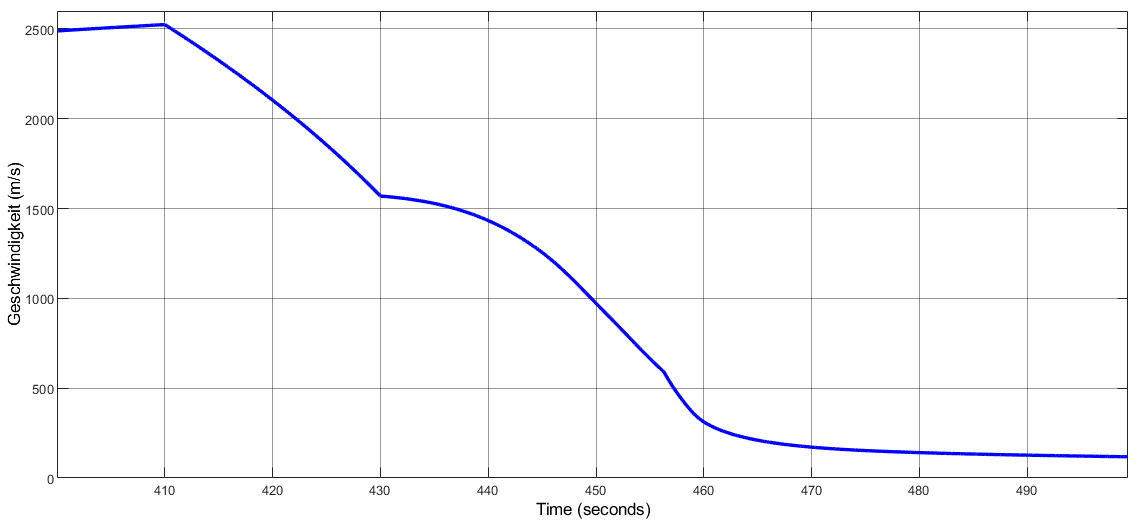
\includegraphics[width=0.9\textwidth]{vNormal.png}
	\caption{Fluggeschwindigkeit bei konstant gehaltener Neutralstellung}
	\label{abb_vNormal}
\end{figure}\\
Dies war nun aber nur ein sehr simpler Missionsablauf, der den Grid Fins nicht viel abverlangt. Für die Auslegung müssen jedoch auch die worst-case-Szenarien berücksichtigt werden. Dazu zählt zum einem ein Ausschlag des Steuerwinkels, wodurch zum einem deutlich höhere Normalkräfte zu Stande kommen, aber auch die Axialkräfte deutlich ansteigen. Des Weiteren ist der Fall zu betrachten, dass der ReEntry-Burn ausfällt, beziehungsweise bewusst weggelassen wird, um die Wirtschaftlichkeit durch geringere Treibstoffmitnahme zu maximieren. In dem Fall würde die Raketenstufe mit deutlich höherer Geschwindigkeit in die Atmosphäre eintauchen, was zu enormen Belastungen führt.

Zu dem maximalen Lastfall kommt es, wenn kein ReEntry-Burn stattfindet und alle Grid Fins um $\eta = \pm 10^\circ$ ausgeschlagen sind. Die Finnen befinden sich dabei in x-Formation und der Ausschlag ist so ausgerichtet, dass ein Moment erzeugt wird, das den Nickwinkel erhöht. Die Kräfte, die in diesem Fall von den Grid Fins ausgehalten werden müssen sind für alle betragsmäßig gleich und in Abbildung \ref{abb_FExtreme} dargestellt. Während die Axialkraft nur leicht ansteigt, nehmen die Normalkräfte sehr hohe Werte an wie der Kraftvektor
\begin{equation}
	\vec{F}(t=440,7\mathrm{s})
	=\left(\begin{array}{c}817\mathrm{N}\\-6530\mathrm{N}\\-6183\mathrm{N}\end{array}\right)
\end{equation}
zeigt. Zu erkennen ist, dass der Wiedereintritt hochfrequenten Schwingungen ausgesetzt die Amplituden von bis zu $\Delta F_z = 3194$N besitzen. Wird nun aber davon ausgegangen, dass eine funktionstüchtige Reglung existiert, so kann diese Schwingung ausgeglichen werden und es käme ein Kraftvektor mit den Mittelwerten zu Stande.
\begin{equation}
\vec{F}_\mathrm{geregelt}(t=440,7\mathrm{s})
=\left(\begin{array}{c}572\mathrm{N}\\-6415\mathrm{N}\\-4995\mathrm{N}\end{array}\right)
\end{equation}
Der Moment, in dem der Ballonschirm deployed ist zwar in diesem Fall deutlich erkennbar, da die Raketenstufe in diesem Moment plötzlich herumgerissen wird, ist jedoch im Vergliech zu den Kräften bei "Max Q"\ vernachlässigbar.
\begin{figure}[h] 
	\centering
	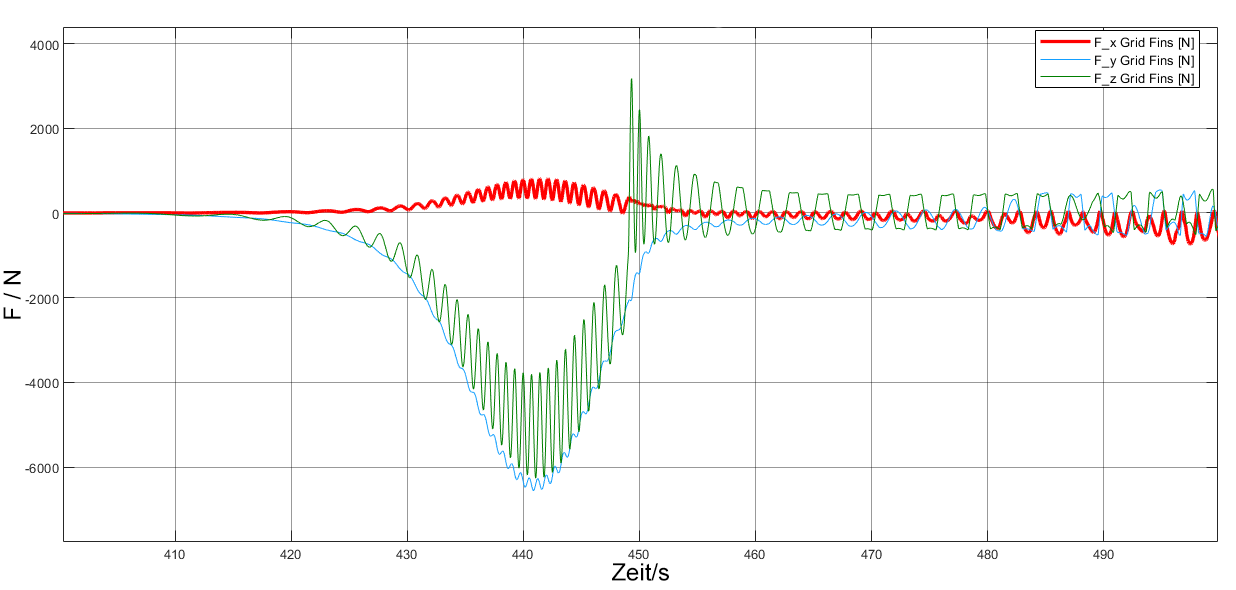
\includegraphics[width=0.9\textwidth]{F2Extreme4.png}
	\caption{Kräfte am Grid Fin beim maximalen Lastfall}
	\label{abb_FExtreme}
\end{figure}\\
\subsection{Geometrische Anforderungen}
Die Hauptmaße der Grid Fins sind hauptsächlich durch die Fertigung begrenzt. Ein Grid Fin soll also in einen entsprechenden 3D-Drucker mit den Maßen $300$x$300$x$400\mathrm{mm}^3$ passen. Für die Größe und Anordnung der Aktuatorik ist darauf zu achten, dass für alle vier Grid Fins jeweils zwei Motoren mit ihren zugehörigen Getrieben in den Raketendurchmesser von $1,1$m passen müssen. Das Innere dieses Durchmessers wird jedoch für die Bordelektronik benötigt, sodass sich die Aktuatorik am äußeren Rand befinden muss. Es ist des Weiteren eine Maximalhöhe von $0,15$m vorgesehen, die nicht überschritten werden darf.
\newpage
\section{Morphologischer Kasten}
Um eine Übersicht über die verschiedenen Designmöglichkeiten zu haben wird an dieser Stelle ein morphologischer Kasten, wie in er in Abbildung \ref{abb_MorphKastGF} zu sehen ist, eingeführt. Für fünf Designentscheidungen des Grid Fins sind dort unterschiedliche Teillösungen aufgelistet. Ganz links sind drei mögliche Zellformen gegeben. Es besteht die Wahl zwischen quadratischen, drei- und sechseckigen Geometrien. Hierbei sei aber wieder zu berücksichtigen, dass es auch zu einer Mischung mehrerer Formen kommen kann und besonders am Rand durch den Rahmen die Zellen ungleichmäßig verkleinert werden könnten.

Für die Form des gesamten Gitters stehen nur drei unterschiedliche Möglichkeiten zur Auswahl: Rechteck, Diamant oder auch eine dem Insektenflügel nachempfundene Struktur. Da jedoch die Maße noch nicht festgelegt sind kann die ersten der beiden Formen auch noch zum Quadrat werden. Des Weiteren kann es sein, dass die Geometrie an der einen Seite für die Anbringung noch angepasst wird.

Die größte Auswahl bietet sich bei den Wandquerschnittsformen. Rechteckig, abgerundet, beidseitig und einseitig spitzt, trapezförmig und dreieckig sind die sechs Optionen, die es hier gibt. Der Wandquerschnitt muss nicht überall die gleiche Form besitzen. So kann es kommen, dass das Gitter eine unterschiedliche erhält als der Rahmen. Die unteren beiden Formen sind zum Beispiel asymmetrisch, sodass sie nur für die Umrandung der Grid Fins in Frage kommen.

Als viertes wird die Fragestellung einer Krümmung gezeigt. Neben einem flachen Design kann der Grid Fin entweder zur Strömung hin konvex oder konkav gekrümmt sein. Dies ist abhängig davon in welche Richtung die Finne eingeklappt werden kann.

Im Grundlagenkapitel wurden drei verschiedene Arten der Pfeilung eines Grid Fins gezeigt. Da sie sich grundsätzlich unterschiedlich implementieren lassen, können sie theoretisch sogar in Kombination gewählt werden. Der Pfeilungswinkel ist für die Varianten noch frei wählbar und auch negative Winkel, also Vorwärtspfeilung, ist denkbar. Für die lokale Pfeilung der Zellen rückt der Unterschied zwischen Vorwärts- und Rückwärtspfeilung durch die Unterscheidung vom Berg- und Tal-Typus noch mehr in den Vordergrund. Wichtig ist noch anzumerken, dass die konfigurelle Pfeilung keinen direkten Einfluss auf das Design der Grid Fins an sich hat, sondern sich durch den Bewegungsspielraum der Aktuatorik umsetzten lässt.
\begin{figure}[h]
	\centering
	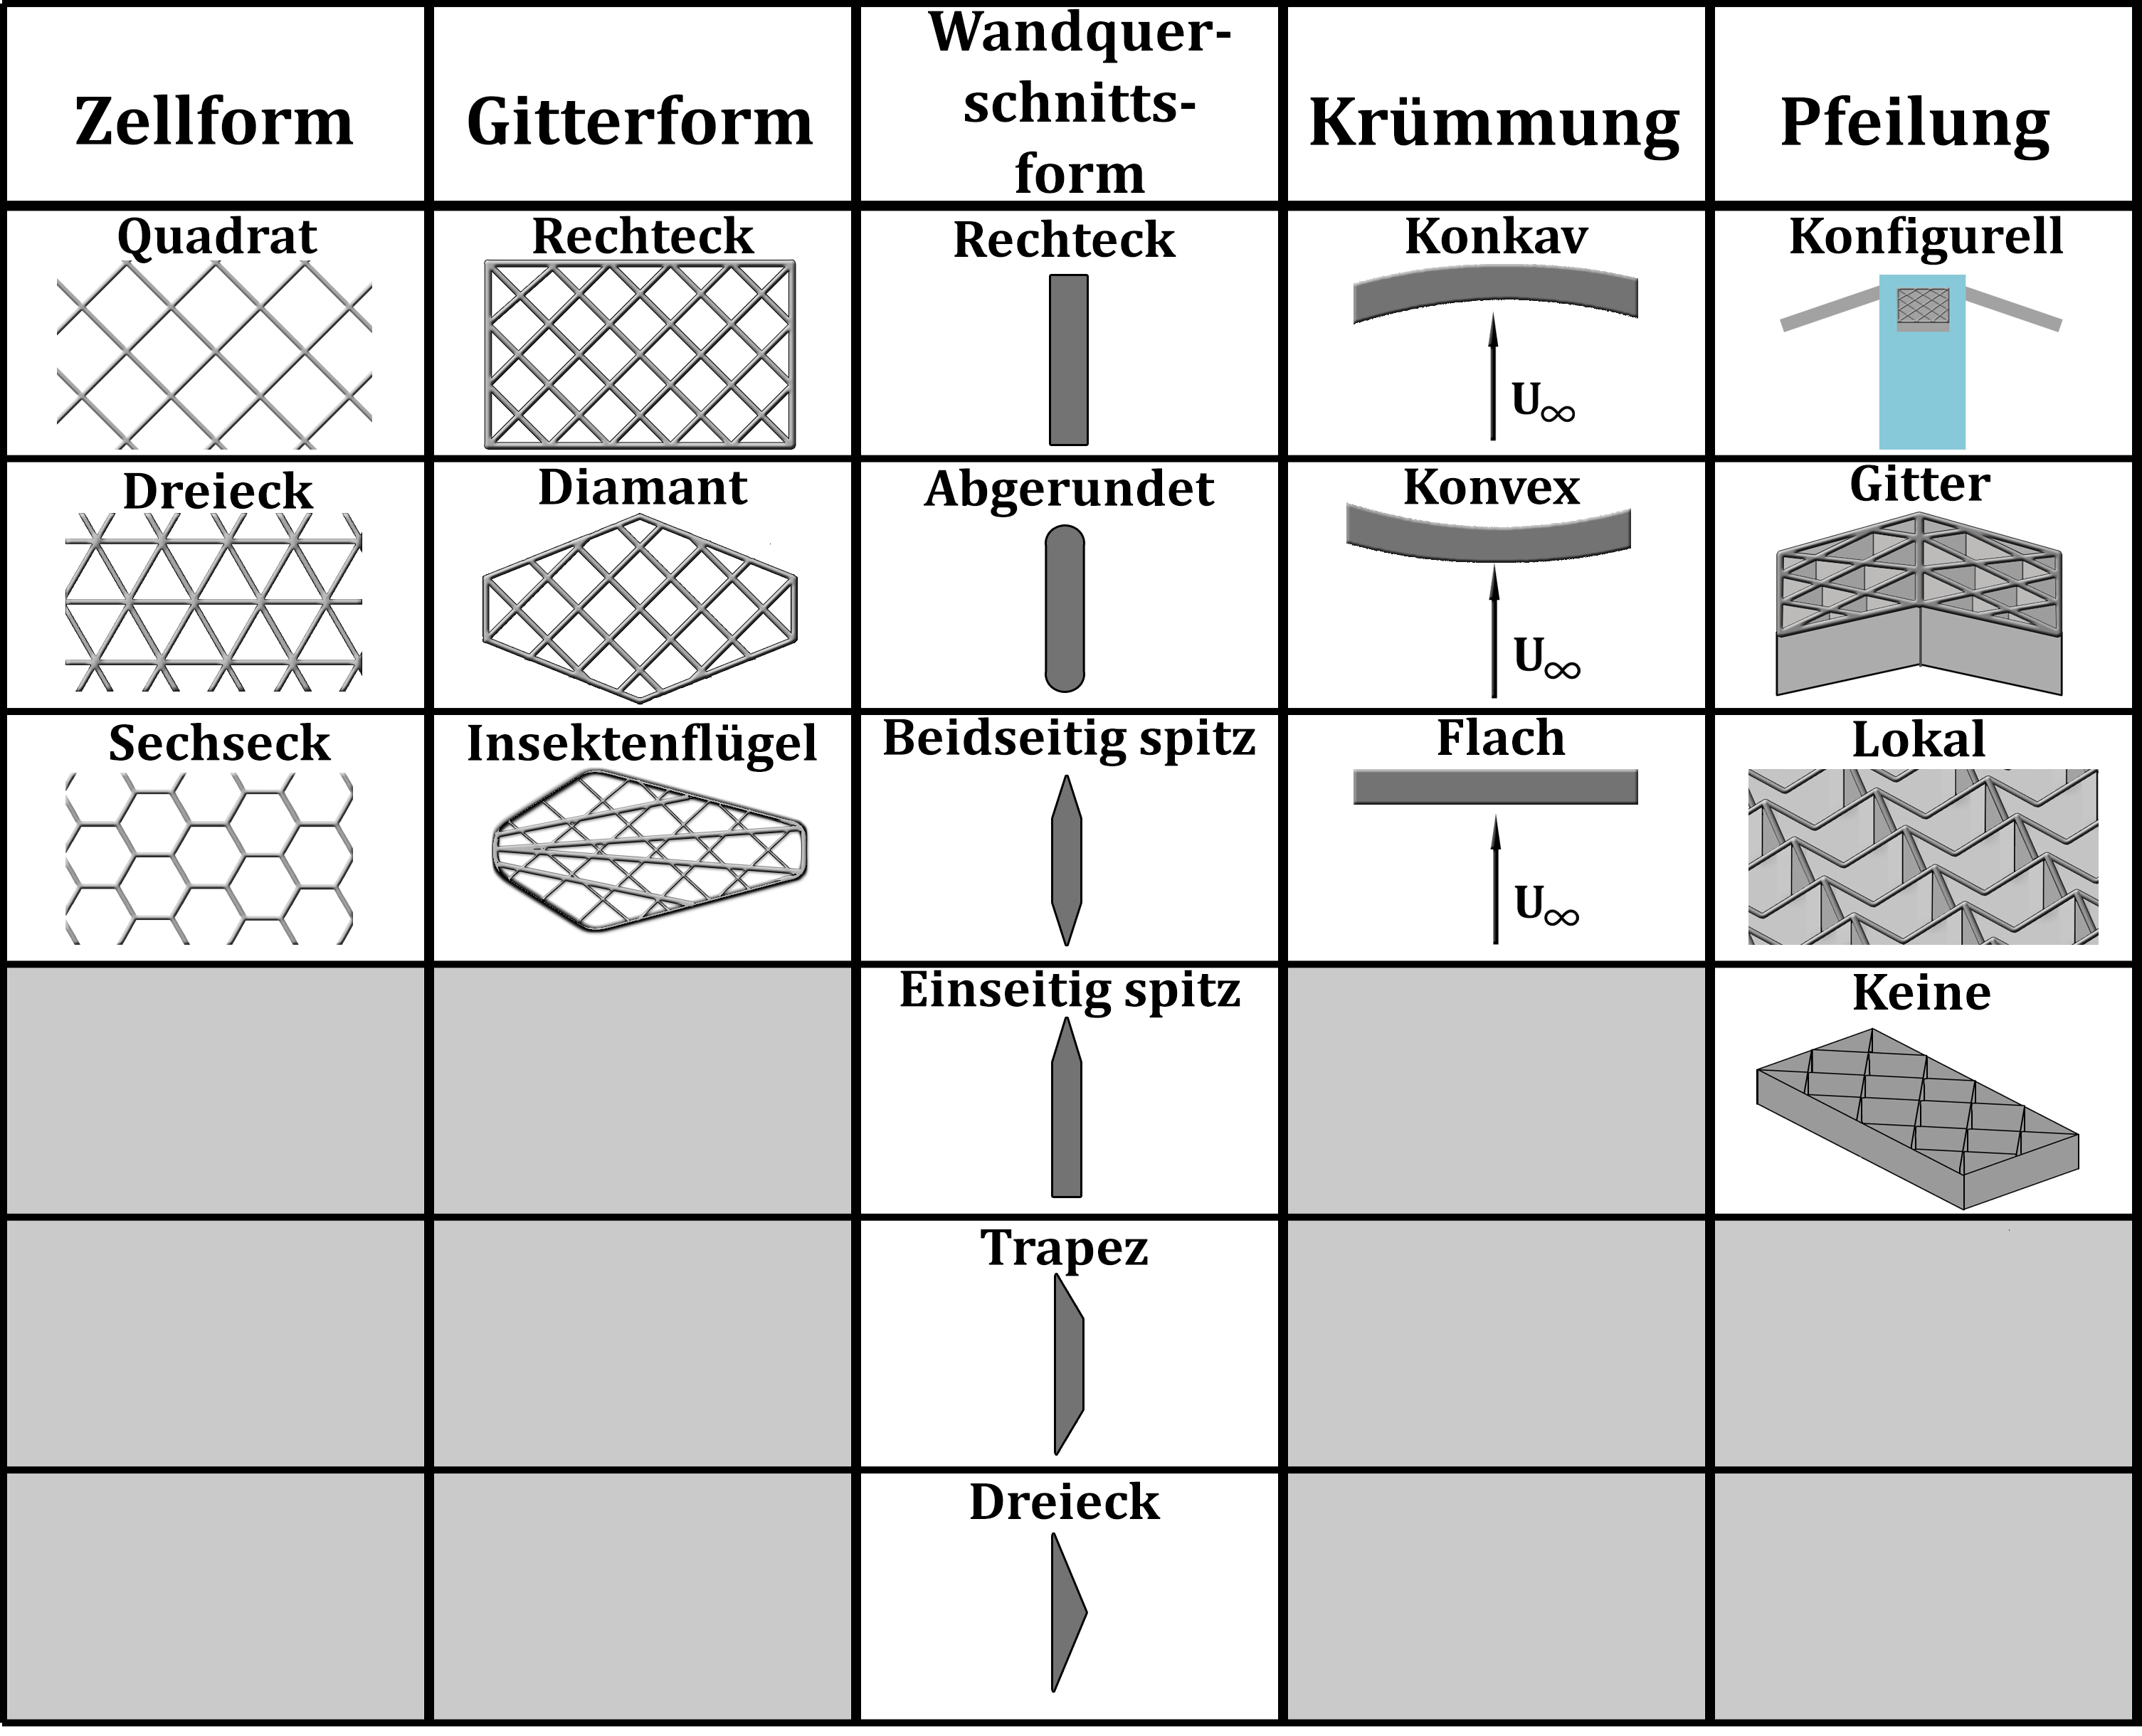
\includegraphics[width=0.9\textwidth]{Morphologischer Kasten GF V2.png}
	\caption{Morphologischer Kasten für die Grid Fins}
	\label{abb_MorphKastGF}
\end{figure}\\~\\
Für den Entwurf der Aktuatorik wurde ein zweiter morphologischer Kasten erstellt. Dieser ist in Abbildung \ref{abb_MorphKastAk} zu sehen und zeigt drei verschieden Designkategorien. Da die Grid Fins zwei unabhängige Freiheitsgrade haben, können für den Steuer- und Klappwinkel separat unterschiedliche Lösungen aus dem morphologischen Kasten gewählt werden.

Eine wichtige Designentscheidung ist der Aktuator, da er bestimmt was als Energiequelle genutzt wird und hat somit einen großen Einfluss auf Gewicht und Kosten. Eine Möglichkeit ist die elektrische Energie zu nutzen und diese mit einem Elektromotor direkt die mechanische Arbeit verrichten zu lassen. Hierbei muss noch die Wahl getroffen werden, ob linear oder rotatorischer Motor vorgezogen werden soll. Alternativ kann auch ein hydraulisches oder gar pneumatisches System verwendet werden. Da Grid Fins zwei Freiheitsgrade haben, können diese über unterschiedliche Aktuatoren, die auch unterschiedlicher Art sein können, bewegt werden. Also muss in diesem Punkt für beide Rotationen einzeln entschieden werden.

Über ein Getriebe wird die Leistung des Aktuators auf die Grid Fins übertragen, um mehr Spielraum für Kraft, Moment, Drehzahl und Orientierung des Aktuators zu gewährleisten. Eine Möglichkeit bietet das klassische Zahnradgetriebe. Viele Paarungen wie Stirn-, Kegel-, Schrauben- oder Schneckenräder sind denkbar. Kräfte und die zugehörige Bewegungsgeschwindigkeit lassen sich auch durch hydrostatische Getriebe beeinflussen. Momente und Drehzahlen können durch hydrodynamische Getriebe verändert werden. Generell sind durch Kombinationen beliebig komplexe Systeme möglich.

Als letztes beschäftigt sich der Morphologische Kasten in Abbildung \ref{abb_MorphKastAk} mit der Lagerung. Hierbei wird generell zwischen den Wälz- und Gleitlagern unterschieden. Beide bieten jedoch noch mehr Entscheidungsfreiheiten. So gibt es einige unterschiedliche Wälzkörper, wie Kugeln, Zylinder, Kegel oder Pendelrollen. Auch Gleitlagern können weiter zu statischen und dynamischen unterteilt werden, je nach Art der Schmierfilmdruckerzeugung.
\begin{figure}[h]
	\centering
	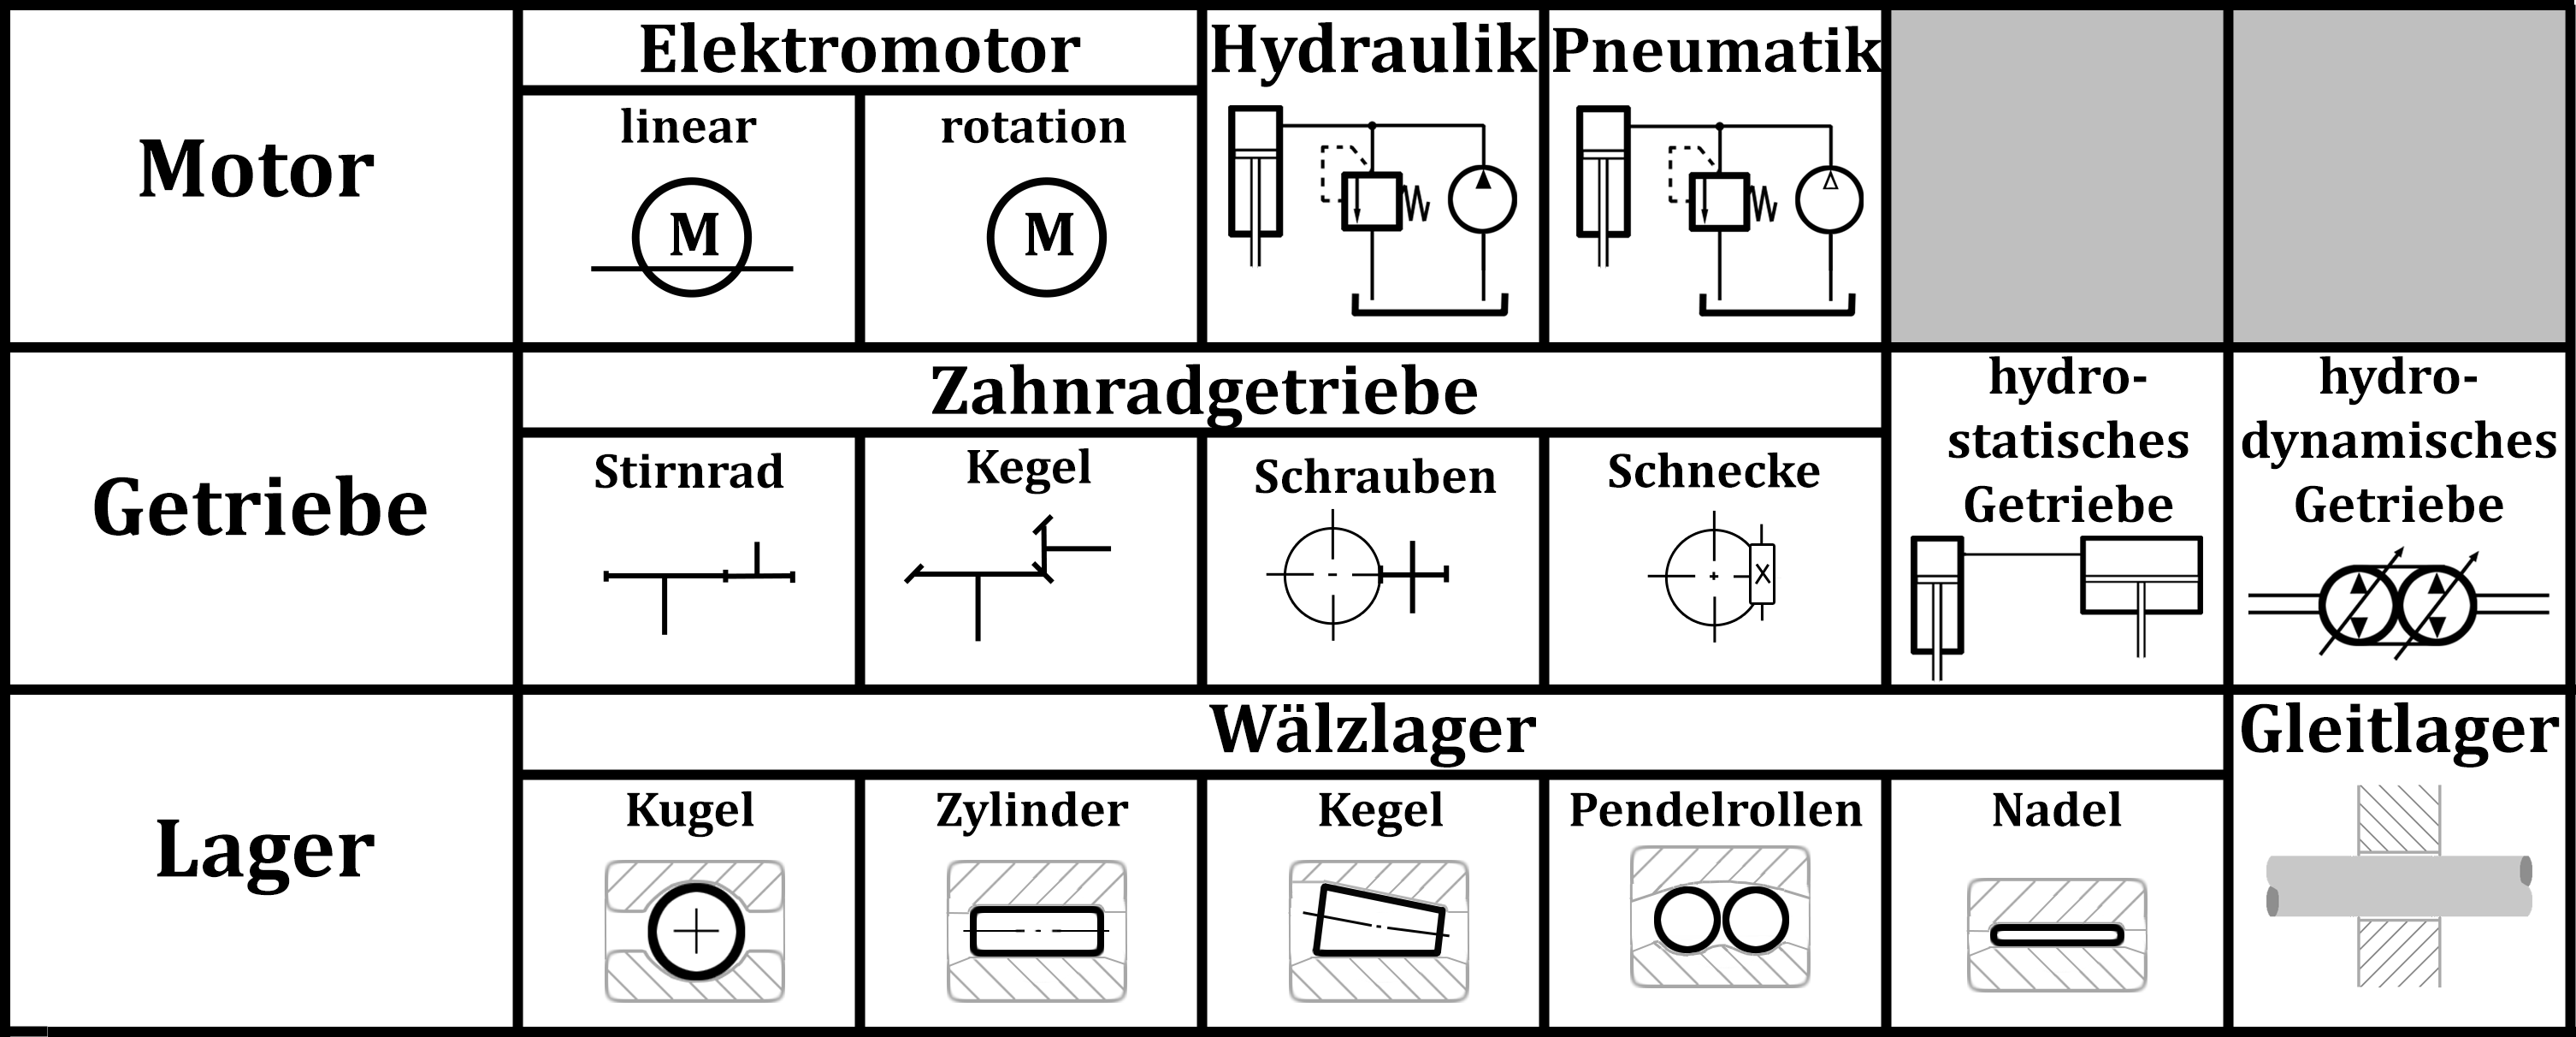
\includegraphics[width=\textwidth]{Morphologischer Kasten Ak.png}
	\caption{Morphologischer Kasten für die Grid Fin Aktuatorik}
	\label{abb_MorphKastAk}
\end{figure}\\
Es gibt jedoch noch weitere Designentscheidungen, die sich nicht in einem morphologischen Kasten pragmatisch darstellen lassen. So müssen zum einen noch die Dimensionen des Moduls und Lage der Aktuatoren in der Rakete definiert werden. Zum anderen stellt sich die Frage welche Zellgröße $g$ und Wandstärke $d$ an welcher Stelle gewählt wird. Es besteht auch noch die Möglichkeit die Grid Fins mit zusätzlichen Features auszustatten. Eine Option wären hier zusätzliche Stützstreben oder sogar durch die additive Fertigung ermöglichte, in das Material integrierte Strukturen, wie zum Beispiel Kühlkanäle oder Drucksensoren.
\newpage
\section{Komponentenrecherche und -auswahl}
Als nächstes werden nun die Ergebnisse der Komponentenrecherche beschrieben und auf Grund der Systemanforderungen mit Hilfe der morphologischen Kästen eine vorläufige Wahl getroffen.
\subsection{Materialwahl}
Für Raumfahrt gibt es eine Vielzahl von Materialien, die in Frage kommen.
\begin{table}[h]
	\centering
	\begin{tabular}{c|c|c|c|c|c|c}
		Werkstoff&Bezeichnung&$\rho$/$\frac{k\mathrm{g}}{\mathrm{cm}^3}$&Preis/€&$T_\mathrm{Einsatz, max}$/$^\circ$C&$T_\mathrm{Schmelz}$/$^\circ$C&$R_{p,0.2}$/MPa\\
		\hline
		Aluminium&AlSi10Mg&2,57&110,48&530&557&230-270\\
		Edelstahl&X2CrNiMo17&7,97&169&850&1400&480-540\\
		Nickel&NiCr22Mo9Nb&8,15&153&950&1350&630-720\\
		Titan&TiAl6V4&4,41&249&>700&1630&1120-1140\\
	\end{tabular}
	\begin{flushright}
	\flushbottom{Quellen: \cite{eos}, \cite{preise}, \cite{T1.1}, \cite{T1.3}, \cite{T1.4}, \cite{T2.1}, \cite{T2.2}, \cite{T2.3}, \cite{T2.4}}
	\end{flushright}
	\caption{Vergleichsdaten der unterschiedlichen Werkstoffe}
\end{table}\label{tab_Werkstoffe} 
\subsection{Gitterdesign}
\subsection{Peripherie}
z.B. Energieversorgung
\subsection{Aktuator}
\subsection{Getriebe und Lagerung}

\section{Festlegung des Modelldesigns}\label{sec:modelldesign}
Gesamtgröße
gap-to-chord
Pfeilungswinkel
Kanäle
Die additive Fertigung des Grid Fins ermöglicht neue Optionen, die für klassische Herstellungsverfahren nicht wirtschaftlich umsetzbar sind. So können zum Beispiel Kanäle in das Material integriert werden, welche genutzt werden können, um den Werkstoff zu kühlen oder gar das Air Flush System mit weiteren Drucksensoren ergänzen.

\section{Modellierung des Modells}